\chapter{Assignment \#8}
\label{ch:ass8n}

\begin{fullwidth}
\begin{enumerate}
\item Use MATLAB's built-in function \lstinline[style=myMatlab]{integral3} to evaluate the integral below.
\begin{equation*}
\int_{-1}^{1} \int_{-1}^{1} \int_{-1}^{1} \left(x^2 + y^2 + z^2\right) \ dx \ dy \ dz
\end{equation*}
Write a function that uses a generalization of the mean value algorithm for Monte Carlo integration, where $\int_{V}f(V)\ dV = \frac{\text{volume of integral bounds}}{N}\sum\limits_{i=1}^{N}f(x_i,y_i,z_i)$; $N$ is the number of sample points and, for this integral, the volume of the integral bounds is 8.  Create a convergence plot to show that the relative error in your Monte Carlo solution---relative to the solution from \lstinline[style=myMatlab]{integral3}---is proportional to $\sfrac{1}{\sqrt{N}}$.

\vspace{1.0cm}


\item In imaging and treatment of breast cancers, an ellipsoidal shape as shown in Figure \ref{fig:ass8n-p2} may be used to represent certain tumors so that changes in their surface areas may be quantified and monitored during treatment.  The surface area of an ellipsoid is given by:
\begin{equation*}
S = 8ab\int_{0}^{\sfrac{\pi}{2}} \ \int_{0}^{\sfrac{\pi}{2}} \ \sin{\theta}\sqrt{1-p\sin^2{\theta}} \ d\theta \ d\phi
\end{equation*}
\begin{figure}[h!]
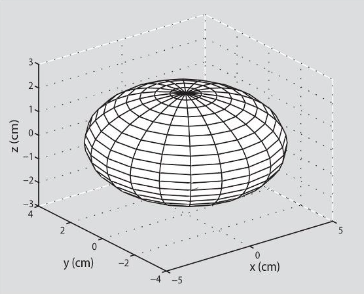
\includegraphics[width=0.5\textwidth]{ass8n-p2.png}
\caption{Elliptical shape for breast cancer.}
\label{fig:ass8n-p2}
\end{figure}
where $p = \delta \sin^2{\phi} + \epsilon \cos^2{\phi}$, $\delta = 1 - \frac{c^2}{a^2}$, $\epsilon = 1 - \frac{c^2}{b^2}$, and $2a$, $2b$, and $2c$ are the major dimensions of the ellipsoid along the $x$, $y$, and $z$ axes, respectively.  For $2a=9.5$ cm, $2b=8$ cm, and $2c=4.2$ cm, calculate the surface area of this ellipsoid tumor using MATLAB built-in functions.


\vspace{1.0cm}


\item Write a user-defined MATLAB function to solve a first-order system of initial value ODEs.  The signature should be \lstinline[style=myMatlab]{[t,y] = odesEULER(F,a,b,N,yINI)} where \lstinline[style=myMatlab]{F} is a handle to a function that defines the system of ODEs, \lstinline[style=myMatlab]{a} and \lstinline[style=myMatlab]{b} are the starting and end points in \lstinline[style=myMatlab]{t}, and \lstinline[style=myMatlab]{yINI} is a vector of initial conditions.  Use this function to solve the following IVP:
\begin{equation*}
\frac{d^2y}{dx^2}+2\frac{dy}{dx} + 2y = 0, \ \ 0<x<1.5, \ y(0)=-1, \ y{\prime}(0) = 0.2
\end{equation*}
The exact solution is: $y(x) = e^{-x}\left(-\cos{(x)} - 4 \sin{(x)}/5\right)$.  Solve the system once for $N=100$ and again for $N=1000$.  Check that your solution exhibits convergence of order 1 using relative error in the 2-norm.

\vspace{1.0cm}

\item Consider the following first-order IVP:
\begin{equation*}
\frac{dy}{dt} = y + t^3, \ \ 0<t<1.5, \ y(0)=1
\end{equation*}
Solve by hand (pencil-paper-calculator) with the classical fourth-order Runge-Kutta method using $h=0.5$.  The analytical solution of the ODE is $y(t)=7e^{t}-t^3 -3t^2 - 6t-6$.  Calculate the error between the true solution and the analytic solution at $t$=0.5, 1.0, and 1.5 seconds.

\vspace{1.0cm}



\item Consider the cylindrical water tank that is shown in Figure \ref{fig:ass8n-p5}.  The tank is being filled at the top, and water flows out of the tank through a pipe that is connected at the bottom.  The rate of change of the height, $h$, of the water is given by the equation below:
\begin{equation*}
\rho \text{A}_{\text{tank}}\frac{dh}{dt} = K_1 + K_2 \sin{(5Ct)}\cos{(Ct)}-\rho \text{A}_{\text{pipe}}\sqrt{2gh}
\end{equation*}
\begin{figure}[h!]
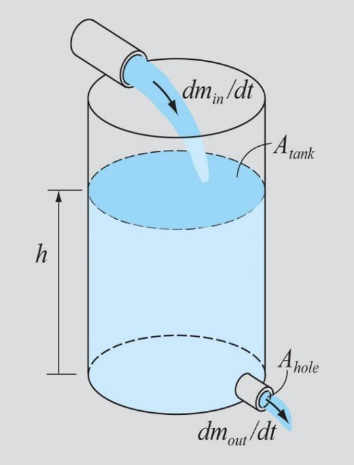
\includegraphics[width=0.4\textwidth]{ass8n-p5.png}
\caption{Water supply tank.}
\label{fig:ass8n-p5}
\end{figure}
For the given tank, $\text{A}_{\text{tank}}=3.13 \ \text{m}^2$, $\text{A}_{\text{pipe}}=0.06 \ \text{m}^2$, $C=\frac{\pi}{12}$, $K_1=300$ kg/s, and, $K_2=1000$ kg/s.  Also, $\rho = 1000$ kg/m$^{3}$, and $g=9.81$ m/s$^{2}$.  Determine and plot the height of the water as a function of time for $0 \le t \le 150$ seconds if, at $t=0$, $h=3m$.
\begin{enumerate}
\item Use the \lstinline[style=myMatlab]{odesEuler} function that you created for problem 3.
\item Create a user defined MATLAB function with signature \lstinline[style=myMatlab]{[t,y] = odesCRK4(F,a,b,N,yINI)} that implements the classical fourth-order Runge-Kutta method.  Use this function to solve the problem.  

\end{enumerate}
For both methods, use N=1000.  In addition to the plot, output the value of $h(150)$ for each method.

Take some time to consider both the given initial value problem, your solution, and its implication on the design of this tank.  What happens when you change the parameters $\text{A}_{\text{tank}}$, $\text{A}_{\text{pipe}}$, $K_1$, $K_2$, and $C$?  Do those changes make sense?  Assuming there are limits on acceptable values of $h$, how does that impact your choice of design parameters such as $\text{A}_{\text{tank}}$ and $\text{A}_{\text{pipe}}$ relative to $K_1$, $K_2$, and $C$?  Write a short discussion (one or two paragraphs, with supporting plots) to present your findings.

\vspace{1.0cm}

\item A small rocket having an initial weight of 3000 lb (including 2400 lb of fuel), and initially at rest, is launched vertically upward.  The rocket burns fuel at a constant rate of 80 lb/s, which provides a constant thrust, $T$, of 8000 lb.  The instantaneous weight of the rocket is $w(t) = 3000 - 80t$ lb.  The drag force, $D$, experienced by the rocket is given by: $D(t) = 0.005g\left(\frac{dy}{dt}\right)^2$ lb, where $y$ is the distance in ft, and $g = 32.2$ ft/s$^2$.  Using Newton's law, the equation of motion for the rocket is given by:
\begin{equation*}
\frac{w}{g}\frac{d^2y}{dt^2}=T-w-D
\end{equation*}
Determine and plot the position, velocity, and acceleration of the rocket (three sets of axes in one figure; use MATLAB's \lstinline[style=myMatlab]{subplot} function) as a function of time from $t=0$, when the rocket starts moving upward from rest, until $t=3$ seconds.  Also, output the distance and velocity at $t=3$ seconds.

Use the user-defined function you created for problem \#5 to solve this equation using the classical fourth-order Runge-Kutta method with $N$=1000.  You may need to adapt the function slightly if you did not initially implement the function to solve systems of equations.  

Take some time to consider the given initial value problem and its solution:
\begin{enumerate}
\item Explain the governing equation and each of its terms.
\item How is the solution different if you do not consider the weight change due to burning of fuel?
\item What happens if the drag force is eliminated?
\item What if the leading term in the drag force is cut in half?  How does this change the shape of the acceleration curve and does this make sense?
\end{enumerate}

Write a short discussion (one or two paragraphs, with supporting plots) to present your findings.

\end{enumerate}

\end{fullwidth}
